% Memoria de calculo analitico (anexo). Generado a partir de memoria_calculo.tex
% ---------- atajos de notación ----------
\newcommand{\ptot}{p_0}\newcommand{\Ttot}{T_0}
\newcommand{\As}{A^{*}}
\newcommand{\dd}{\,\mathrm{d}}
\newcommand{\Msone}{M_{s1}}\newcommand{\Mstwo}{M_{s2}}
\newcommand{\ie}{es decir,\ }

\lstset{basicstyle=\ttfamily\footnotesize,breaklines=true,frame=single,numbers=left,
        numberstyle=\tiny,keywordstyle=\bfseries,language=Python,columns=fullflexible,
        inputencoding=utf8,extendedchars=true,
        literate={á}{{\'a}}1 {é}{{\'e}}1 {í}{{\'i}}1 {ó}{{\'o}}1 {ú}{{\'u}}1 {ñ}{{\~n}}1}

\subsection{Objetivo y alcance}
%=====================================================================
Esta memoria desarrolla, paso a paso y sin saltar álgebra, el modelo analítico
cuasiunidimensional que se usa como referencia para validar las simulaciones CFD
(Gmsh + OpenFOAM-8, solver \texttt{rhoCentralFoam}) de una tobera convergente-divergente
de relación de áreas $A_e/A_t=\ARr$. Se resuelven tres regímenes internos (Nivel~1):

\begin{itemize}[leftmargin=2em]
\item \textbf{S}: subsónico no estrangulado ($M_t<1$ en la garganta),
\item \textbf{A}: supersónico adaptado (garganta sónica, divergente supersónico, $p_e=p_{e,is}$),
\item \textbf{C}: choque normal interno en el divergente.
\end{itemize}

Para cada régimen se obtienen los perfiles $M(x)$, $p(x)/p_{01}$, $T(x)/T_{01}$, el gasto
másico y el estado de salida $(M_e,p_e,T_e,V_e)$ usando la \emph{distribución real} $A(x)$ de la
geometría construida en Gmsh (no una distribución idealizada). En el caso C se obtienen además
$A_s/A_t$, $x_s/L_d$, $M_{s1}$, $M_{s2}$, $p_2/p_1$ y $p_{02}/p_{01}$.

\textbf{Convención de índices.} Subíndice 0: condición de estancamiento (total); subíndice 1:
alimentación (entrada); $t$: garganta geométrica; $e$: salida; $s$: estación del choque; en el choque,
$1$ es aguas arriba y $2$ aguas abajo (se escribe $M_{s1}$, $M_{s2}$ para evitar confusión con el
subíndice de alimentación $p_{01},T_{01}$). El símbolo $A^{*}$ denota el \emph{área crítica}
(el área que tendría la sección si el flujo isentrópico alcanzara $M=1$), que \textbf{no} es
en general igual al área geométrica de garganta $A_t$ (véanse los casos S y C).

%=====================================================================
\subsection{Hipótesis}
%=====================================================================
\begin{enumerate}[label=\textbf{H\arabic*.},leftmargin=2.2em]
\item Flujo \textbf{cuasiunidimensional}: las propiedades dependen sólo de $x$ y el área de la sección
  $A(x)$ varía lentamente. La pendiente máxima de la pared del contorno elegido es pequeña
  (pendiente cero en la garganta y en la salida), lo que hace razonable la hipótesis.
\item Flujo \textbf{estacionario}.
\item Gas \textbf{perfecto} y calóricamente perfecto: $p=\rho R T$, $c_p$ y $\gamma$ constantes;
  aire con $\gamma=\gam$, $R=\Rgas\ \mathrm{J/(kg\,K)}$, $c_p=\gamma R/(\gamma-1)=1004.5\ \mathrm{J/(kg\,K)}$.
\item Flujo \textbf{adiabático e inviscido} (Nivel~1 de la hoja de actividad): paredes impermeables y
  deslizantes, sin capa límite. Entonces $T_0$ es constante a lo largo de todo el flujo, incluso a través del choque.
\item Flujo \textbf{isentrópico} excepto a través del choque normal (caso C); $p_0$ constante antes y
  después del choque, pero con un salto $p_{02}<p_{01}$ en el choque.
\item Dominio \textbf{2D planar}: profundidad $b$ constante en $z$. Con semialtura $h(x)$ y plano de simetría, el área
  de la sección completa es $A(x)=2\,b\,h(x)$; la relación de áreas es entonces
  $A/A_t=h/h_t$ y no depende de $b$. En el modelo numérico se simula la mitad superior con
  $b=\dzz$~m (una celda en $z$).
\item Alimentación de reservorio a $p_{01}=\pu$~kPa, $T_{01}=\Tu$~K, velocidad despreciable en
  el reservorio (parámetros \textbf{provisionales}, a justificar en el reporte).
\end{enumerate}

%=====================================================================
\subsection{Parámetros y geometría real $A(x)$}
%=====================================================================
La geometría de \texttt{tobera.geo} (Gmsh) usa dos tramos con perfil de coseno, con garganta en $x=0$:

\begin{align}
 \text{Convergente } (-L_c\le x\le 0):\quad h(x) &= h_t+\frac{h_i-h_t}{2}\left[1+\cos\!\left(\pi\,\frac{x+L_c}{L_c}\right)\right], \label{m:eq:hconv}\\
 \text{Divergente } (0\le x\le L_d):\quad h(x) &= h_t+\frac{h_e-h_t}{2}\left[1-\cos\!\left(\pi\,\frac{x}{L_d}\right)\right]. \label{m:eq:hdiv}
\end{align}

\textbf{Verificación de los extremos.}
En el convergente: para $x=-L_c$, $\cos(0)=1$ y $h=h_t+(h_i-h_t)=h_i$. Para $x=0$,
$\cos(\pi)=-1$ y $h=h_t$. En el divergente: para $x=0$, $\cos 0=1$ y $h=h_t$; para $x=L_d$, $\cos\pi=-1$
y $h=h_t+(h_e-h_t)=h_e$. La derivada en la garganta es $\mathrm{d}h/\mathrm{d}x=-\tfrac{\pi(h_i-h_t)}{2L_c}\sin(\pi)=0$
por el lado convergente y $\tfrac{\pi(h_e-h_t)}{2L_d}\sin(0)=0$ por el divergente: la pared es suave ($C^1$) en la garganta;
también $\mathrm{d}h/\mathrm{d}x=0$ en $x=L_d$.

\begin{table}[H]\centering
\caption{Parámetros geométricos y de alimentación (provisionales).}\label{m:tab:param}
\begin{tabular}{lcc}\toprule
Parámetro & Símbolo & Valor\\\midrule
Semialtura de garganta & $h_t$ & \hth\ m\\
Semialtura de salida & $h_e=\ARr\,h_t$ & \heh\ m\\
Semialtura de entrada & $h_i=3h_t$ & \hih\ m\\
Longitud del convergente & $L_c$ & \Lcc\ m\\
Longitud del divergente & $L_d$ & \Ldd\ m\\
Relación de áreas asignada & $A_e/A_t=h_e/h_t$ & \ARr\\
Presión total de alimentación & $p_{01}$ & \pu\ kPa\\
Temperatura total de alimentación & $T_{01}$ & \Tu\ K\\
Gas (aire) & $\gamma$, $R$ & \gam, \Rgas\ J/(kg K)\\\bottomrule
\end{tabular}\end{table}

\textbf{Comprobación de la relación de áreas:} $A_e/A_t=h_e/h_t=\heh/\hth=\ARr$. \checkmark

\begin{table}[H]\centering
\caption{Distribución real $A(x)/A_t=h(x)/h_t$ en estaciones seleccionadas.}\label{m:tab:geom}
\begin{tabular}{ccc}
\toprule
$x$ [m] & $h(x)$ [m] & $A/A_t=h/h_t$ \\
\midrule
-0.25 & 0.07500 & 3.0000 \\
-0.20 & 0.07023 & 2.8090 \\
-0.15 & 0.05773 & 2.3090 \\
-0.10 & 0.04227 & 1.6910 \\
-0.05 & 0.02977 & 1.1910 \\
+0.00 & 0.02500 & 1.0000 \\
+0.05 & 0.02720 & 1.0879 \\
+0.10 & 0.03250 & 1.3000 \\
+0.15 & 0.03780 & 1.5121 \\
+0.20 & 0.04000 & 1.6000 \\
\bottomrule
\end{tabular}\end{table}

\begin{figure}[H]\centering
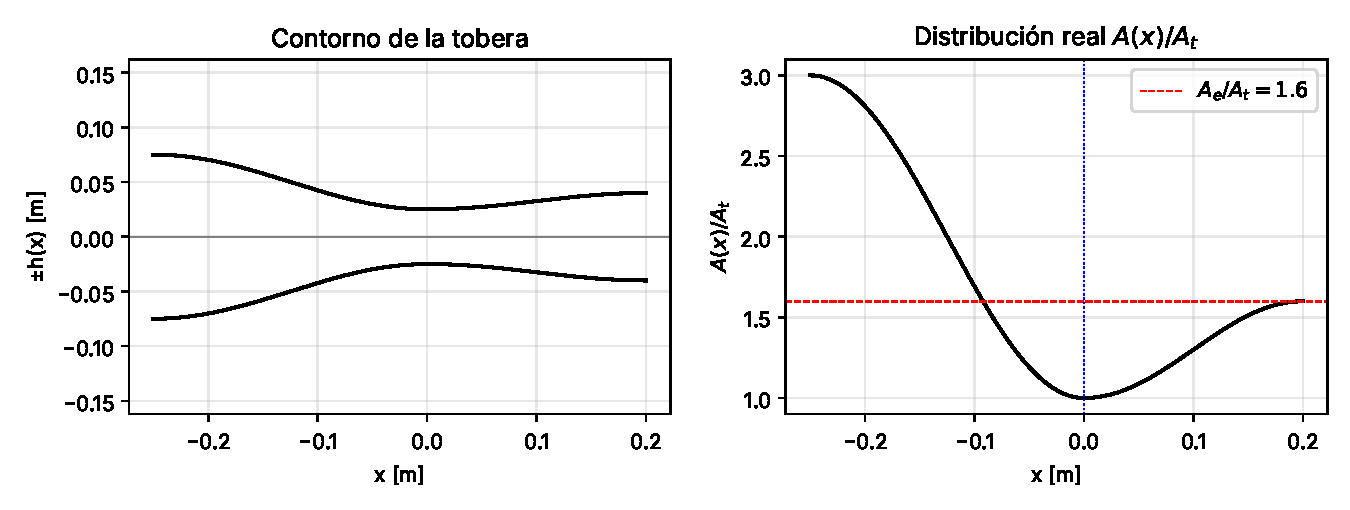
\includegraphics[width=\textwidth]{memoria/figuras/geometria_Ax.pdf}
\caption{Contorno de la tobera (semialtura $\pm h(x)$) y distribución real de áreas $A(x)/A_t$.}
\label{m:fig:geom}\end{figure}

\textbf{Inversa en el divergente.} Para localizar el choque se necesita conocer $x$ a partir de
$A/A_t$. Escribiendo $a\equiv A/A_t=h/h_t$ en \eqref{m:eq:hdiv}:
$a=1+\frac{h_e-h_t}{2h_t}\left[1-\cos(\pi x/L_d)\right]=1+\frac{A_e/A_t-1}{2}\left[1-\cos(\pi x/L_d)\right]$.
Despejando,
\begin{equation}
\cos\!\left(\frac{\pi x}{L_d}\right)=1-\frac{2\,(a-1)}{A_e/A_t-1}
\quad\Longrightarrow\quad
x(a)=\frac{L_d}{\pi}\arccos\!\left[1-\frac{2\,(a-1)}{A_e/A_t-1}\right],\quad 0\le x\le L_d. \label{m:eq:xinv}
\end{equation}
En $[0,L_d]$ la función $\cos(\pi x/L_d)$ es monótona decreciente, por lo que la inversa es única.

%=====================================================================
\subsection{Relaciones isentrópicas}
%=====================================================================
\subsubsection{Temperatura total}
Para un gas calóricamente perfecto, la ecuación de energía de un flujo adiabático estacionario
($h+V^2/2=h_0$ con $h=c_pT$) da
$c_pT+\tfrac12V^2=c_pT_0$. Dividiendo entre $c_pT$ y usando $c_p=\gamma R/(\gamma-1)$ y $a^2=\gamma RT$:
\[
\frac{T_0}{T}=1+\frac{V^2}{2c_pT}=1+\frac{V^2(\gamma-1)}{2\gamma RT}=1+\frac{\gamma-1}{2}M^2,
\]
\begin{equation}
\boxed{\frac{T}{T_0}=\left(1+k\,M^2\right)^{-1},\qquad k\equiv\frac{\gamma-1}{2}=\kk}\label{m:eq:T}
\end{equation}

\subsubsection{Presión y densidad}
En un proceso isentrópico $p/\rho^{\gamma}=\text{cte}$ y $p=\rho RT$, de donde $p\propto T^{\gamma/(\gamma-1)}$ y
$\rho\propto T^{1/(\gamma-1)}$. Con \eqref{m:eq:T}:
\begin{equation}
\boxed{\frac{p}{p_0}=\left(1+kM^2\right)^{-\gamma/(\gamma-1)},\qquad
\frac{\rho}{\rho_0}=\left(1+kM^2\right)^{-1/(\gamma-1)}}\label{m:eq:prho}
\end{equation}
Para $\gamma=\gam$: los exponentes son $-\gamma/(\gamma-1)=-3.5$ y $-1/(\gamma-1)=-2.5$.
Inversa útil (para obtener $M$ a partir de una presión conocida):
\begin{equation}
M=\sqrt{\frac{1}{k}\left[\left(\frac{p_0}{p}\right)^{(\gamma-1)/\gamma}-1\right]}. \label{m:eq:Mdep}
\end{equation}

\subsubsection{Condiciones críticas ($M=1$)}
De \eqref{m:eq:T}--\eqref{m:eq:prho} con $M=1$ y $1+k=(\gamma+1)/2$:
\[
\frac{T^*}{T_0}=\frac{2}{\gamma+1}=0.8333,\qquad
\frac{p^*}{p_0}=\left(\frac{2}{\gamma+1}\right)^{\gamma/(\gamma-1)}=0.5283,\qquad
\frac{\rho^*}{\rho_0}=\left(\frac{2}{\gamma+1}\right)^{1/(\gamma-1)}=0.6339.
\]
Con $T_0=\Tu$~K y $p_0=\pu$~kPa: $\rho_0=p_0/(RT_0)=\rhocero$~kg/m$^3$,
$\rho^*=\rhostar$~kg/m$^3$ y $a^*=\sqrt{2\gamma RT_0/(\gamma+1)}=\astar$~m/s.

%=====================================================================
\subsection{Relación área--Mach}
%=====================================================================
\subsubsection{Derivación}
La conservación de masa para flujo estacionario cuasi-1D es $\dot m=\rho VA=\text{cte}$. Aplicada entre una sección
cualquiera ($M$, $A$) y la sección crítica ($M=1$, $A=\As$) del \emph{mismo} flujo isentrópico:
\[
\rho V A=\rho^*V^*\As
\quad\Longrightarrow\quad
\frac{A}{\As}=\frac{\rho^*V^*}{\rho V}=\frac{\rho^*}{\rho}\cdot\frac{a^*}{M\,a}.
\]
Se expresa cada cociente con \eqref{m:eq:T}--\eqref{m:eq:prho}. Como $\rho_0$ y $T_0$ son iguales en ambas secciones,
\[
\frac{\rho^*}{\rho}=\frac{\rho^*/\rho_0}{\rho/\rho_0}=\frac{\left(1+k\right)^{-1/(\gamma-1)}}{\left(1+kM^2\right)^{-1/(\gamma-1)}}=\left(\frac{1+kM^2}{1+k}\right)^{1/(\gamma-1)},
\qquad
\frac{a^*}{a}=\sqrt{\frac{T^*}{T}}=\left(\frac{1+kM^2}{1+k}\right)^{1/2}.
\]
Multiplicando, los exponentes se suman: $\dfrac{1}{\gamma-1}+\dfrac12=\dfrac{2+(\gamma-1)}{2(\gamma-1)}=\dfrac{\gamma+1}{2(\gamma-1)}$. Por tanto
\begin{equation}
\boxed{\frac{A}{\As}=\frac{1}{M}\left[\frac{1+kM^2}{1+k}\right]^{\frac{\gamma+1}{2(\gamma-1)}}
=\frac{1}{M}\left[\frac{2}{\gamma+1}\left(1+\frac{\gamma-1}{2}M^2\right)\right]^{\frac{\gamma+1}{2(\gamma-1)}}}\label{m:eq:AM}
\end{equation}
(la segunda forma usa $1/(1+k)=2/(\gamma+1)$). Con $\gamma=\gam$ el exponente es $3$.

\subsubsection{Propiedades: dos ramas y mínimo en $M=1$}
Derivando $\ln(A/\As)$ respecto de $M$:
\[
\frac{\dd\ln(A/\As)}{\dd M}=-\frac{1}{M}+\frac{\gamma+1}{2(\gamma-1)}\cdot\frac{2kM}{1+kM^2}
=-\frac1M+\frac{(\gamma+1)M}{2(1+kM^2)}
=\frac{-2(1+kM^2)+(\gamma+1)M^2}{2M(1+kM^2)}.
\]
Como $2k=\gamma-1$, el numerador es $-2-(\gamma-1)M^2+(\gamma+1)M^2=2(M^2-1)$. Entonces
\begin{equation}
\boxed{\frac{\dd(A/\As)}{\dd M}=\frac{A}{\As}\cdot\frac{M^2-1}{M\left(1+kM^2\right)}}\label{m:eq:dAM}
\end{equation}
\textbf{Conclusión:} $A/\As$ decrece para $M<1$, tiene un mínimo igual a $1$ en $M=1$ y crece para $M>1$. Por eso, para un valor dado
$A/\As>1$ existen \emph{dos} soluciones $M$: una subsónica y una supersónica. La rama correcta se elige por la historia del flujo:
subsónica en el convergente; en el divergente, supersónica si la garganta es sónica y no hay choque aguas arriba,
y subsónica después de un choque normal.

\subsubsection{Solución numérica: método de Newton--Raphson}
\eqref{m:eq:AM} es trascendente en $M$ y no se puede despejar en forma cerrada para $\gamma$ general. Se resuelve
$f(M)\equiv A/\As(M)-a=0$ con Newton--Raphson, usando la derivada exacta \eqref{m:eq:dAM}:
\[
M_{n+1}=M_n-\frac{f(M_n)}{f'(M_n)}=M_n-\frac{A/\As(M_n)-a}{\left.A/\As\right|_{M_n}\,(M_n^2-1)/[M_n(1+kM_n^2)]}.
\]
Se detiene cuando $|M_{n+1}-M_n|<10^{-13}$. \textbf{Elección de la semilla:} se toma $M_0=2$ para la rama supersónica y $M_0=0.4$--$0.5$ para la
subsónica, lejos de $M=1$ donde $f'=0$ (allí el método falla porque la derivada se anula).
Newton converge cuadráticamente: el número de cifras correctas se duplica en cada iteración (véanse las tablas).

\subsubsection{Resultado para $A_e/A_t=\ARr$}
\textbf{Rama supersónica} ($M_0=2$, tabla~\ref{m:tab:nsup}) y \textbf{rama subsónica} ($M_0=0.4$, tabla~\ref{m:tab:nsub}):
\[
M_e^{\rm sup}=\MeSup,\qquad M_e^{\rm sub}=\MeSub .
\]
Sustituyendo en \eqref{m:eq:prho} y \eqref{m:eq:T}: $p_e/p_{01}=\peSup$ y $T_e/T_{01}=\TeSup$ en la rama supersónica;
$p_e/p_{01}=\peSubr$ y $T_e/T_{01}=\TeSubr$ en la rama subsónica.

\begin{table}[H]\centering\small
\caption{Newton--Raphson, rama supersónica ($A/\As=\ARr$, $M_0=2$).}\label{m:tab:nsup}
\begin{tabular}{rcccc}
\toprule
$n$ & $M_n$ & $f(M_n)=A/A^*(M_n)-1.6$ & $f'(M_n)$ & $\Delta M_n=-f/f'$ \\
\midrule
0 & 2.0000000000 & 8.750e-02 & 1.406250 & -6.222e-02 \\
1 & 1.9377777778 & 3.276e-03 & 1.301781 & -2.516e-03 \\
2 & 1.9352616065 & 5.189e-06 & 1.297657 & -3.999e-06 \\
3 & 1.9352576078 & 1.309e-11 & 1.297651 & -1.009e-11 \\
4 & 1.9352576078 & 8.882e-16 & 1.297651 & -6.845e-16 \\
\bottomrule
\end{tabular}\end{table}
\begin{table}[H]\centering\small
\caption{Newton--Raphson, rama subsónica ($A/\As=\ARr$, $M_0=0.4$).}\label{m:tab:nsub}
\begin{tabular}{rcccc}
\toprule
$n$ & $M_n$ & $f(M_n)=A/A^*(M_n)-1.6$ & $f'(M_n)$ & $\Delta M_n=-f/f'$ \\
\midrule
0 & 0.4000000000 & -9.860e-03 & -3.235750 & -3.047e-03 \\
1 & 0.3969527930 & 8.541e-05 & -3.292017 & 2.594e-05 \\
2 & 0.3969787361 & 6.284e-09 & -3.291533 & 1.909e-09 \\
3 & 0.3969787380 & -6.661e-16 & -3.291533 & -2.024e-16 \\
\bottomrule
\end{tabular}\end{table}

%=====================================================================
\subsection{Gasto másico bloqueado}
%=====================================================================
Con garganta sónica, el gasto es el de las condiciones críticas: $\dot m=\rho^*a^*A_t$. Usando
$\rho^*=\rho_0\left(\tfrac{2}{\gamma+1}\right)^{1/(\gamma-1)}$, $\rho_0=p_0/(RT_0)$ y
$a^*=\sqrt{\tfrac{2}{\gamma+1}\gamma RT_0}$:
\[
\dot m=A_t\,\frac{p_0}{RT_0}\sqrt{\frac{2\gamma RT_0}{\gamma+1}}\left(\frac{2}{\gamma+1}\right)^{\frac{1}{\gamma-1}}
=A_t\,p_0\sqrt{\frac{\gamma}{RT_0}}\;\sqrt{\frac{2}{\gamma+1}}\left(\frac{2}{\gamma+1}\right)^{\frac{1}{\gamma-1}}.
\]
Los exponentes de $\tfrac{2}{\gamma+1}$ suman $\tfrac12+\tfrac1{\gamma-1}=\tfrac{\gamma+1}{2(\gamma-1)}$:
\begin{equation}
\boxed{\dot m=A_t\,p_0\sqrt{\frac{\gamma}{RT_0}}\left(\frac{2}{\gamma+1}\right)^{\frac{\gamma+1}{2(\gamma-1)}}}\label{m:eq:mdot}
\end{equation}
Numéricamente, $\sqrt{\gamma/(RT_0)}\,(2/(\gamma+1))^{3}=\coefm\ \mathrm{s/m}$, con lo que
\[
\dot m'\equiv\frac{\dot m}{b}=2h_t\,p_{01}\cdot\coefm=\mathbf{\mdotfull}\ \mathrm{kg/(s\,m)}
\quad\text{(por metro de profundidad, tobera completa).}
\]
Para el semidominio simulado ($A_t=h_t\,b$, $b=\dzz$~m): $\dot m=\mdotsemi$~kg/s. \emph{Este es el valor de
referencia para el gasto del CFD en los casos A y C.} Mientras la garganta esté sónica, el gasto no depende de la contrapresión.

%=====================================================================
\subsection{Choque normal}
%=====================================================================
\subsubsection{Ecuaciones}
Sea un choque normal estacionario con estado 1 (aguas arriba, supersónico) y 2 (aguas abajo). Sea $r\equiv\rho_2/\rho_1=V_1/V_2$ (continuidad),
$\Pi\equiv p_2/p_1$. Se usan $a^2=\gamma p/\rho$ y $V_1^2=M_1^2\,\gamma p_1/\rho_1$.

\begin{align}
\text{Continuidad:}&\quad \rho_1V_1=\rho_2V_2\ \Rightarrow\ r=V_1/V_2,\\
\text{Cantidad de movimiento:}&\quad p_1+\rho_1V_1^2=p_2+\rho_2V_2^2,\\
\text{Energía:}&\quad \tfrac{\gamma}{\gamma-1}\tfrac{p_1}{\rho_1}+\tfrac12V_1^2=\tfrac{\gamma}{\gamma-1}\tfrac{p_2}{\rho_2}+\tfrac12V_2^2.
\end{align}

\textbf{Paso 1 (momento).} De la cantidad de movimiento y $V_2=V_1/r$: $p_2-p_1=\rho_1V_1^2(1-1/r)$. Dividiendo entre $p_1$ y usando $\rho_1V_1^2/p_1=\gamma M_1^2$:
\begin{equation}\Pi-1=\gamma M_1^2\left(1-\frac1r\right).\label{m:eq:mom}\end{equation}

\textbf{Paso 2 (energía).} Dividiendo la energía entre $\gamma p_1/\rho_1$ y usando $p_2/\rho_2=(p_1/\rho_1)\,\Pi/r$ y $V_1^2/(\gamma p_1/\rho_1)=M_1^2$:
\[
\frac{1}{\gamma-1}\left(1-\frac{\Pi}{r}\right)+\frac{M_1^2}{2}\left(1-\frac1{r^2}\right)=0
\ \Longrightarrow\
\frac{\Pi}{r}-1=\frac{\gamma-1}{2}M_1^2\left(1-\frac1{r^2}\right).\label{m:eq:en}
\]

\textbf{Paso 3 (eliminar $\Pi$).} Se sustituye \eqref{m:eq:mom} en el lado izquierdo de la ecuación de energía:
\[
\frac{\Pi}{r}-1=\frac1r+\gamma M_1^2\left(\frac1r-\frac1{r^2}\right)-1=-\left(1-\frac1r\right)+\gamma M_1^2\,\frac1r\left(1-\frac1r\right)
=\left(1-\frac1r\right)\left[\frac{\gamma M_1^2}{r}-1\right].
\]
El lado derecho se factoriza como $\tfrac{\gamma-1}{2}M_1^2\left(1-\tfrac1r\right)\left(1+\tfrac1r\right)$. Para un choque no trivial ($r\ne1$) se
\textbf{factoriza y cancela} $(1-1/r)$:
\[
\frac{\gamma M_1^2}{r}-1=\frac{\gamma-1}{2}M_1^2\left(1+\frac1r\right).
\]
Multiplicando por $2r$: $2\gamma M_1^2-2r=(\gamma-1)M_1^2\,r+(\gamma-1)M_1^2$, y agrupando los términos en $r$:
$\left[2\gamma-(\gamma-1)\right]M_1^2=r\left[(\gamma-1)M_1^2+2\right]$, con $2\gamma-(\gamma-1)=\gamma+1$:
\begin{equation}
\boxed{\frac{\rho_2}{\rho_1}=r=\frac{(\gamma+1)M_1^2}{(\gamma-1)M_1^2+2}}\label{m:eq:rho}
\end{equation}

\textbf{Paso 4 (presión).} Sustituyendo \eqref{m:eq:rho} en \eqref{m:eq:mom}, con $1-1/r=\dfrac{r-1}{r}$ y
$r-1=\dfrac{(\gamma+1)M_1^2-(\gamma-1)M_1^2-2}{(\gamma-1)M_1^2+2}=\dfrac{2(M_1^2-1)}{(\gamma-1)M_1^2+2}$:
$\dfrac{r-1}{r}=\dfrac{2(M_1^2-1)}{(\gamma+1)M_1^2}$, y por tanto
\begin{equation}
\boxed{\frac{p_2}{p_1}=\Pi=1+\frac{2\gamma}{\gamma+1}\left(M_1^2-1\right)}\label{m:eq:pres}
\end{equation}

\textbf{Paso 5 (Mach aguas abajo).} $M_2^2=V_2^2\rho_2/(\gamma p_2)=\dfrac{V_1^2/r^2}{\gamma p_1\Pi/\rho_1\cdot r}=\dfrac{M_1^2}{r\,\Pi}$. Multiplicando \eqref{m:eq:rho}
por \eqref{m:eq:pres} (con $\Pi=[2\gamma M_1^2-(\gamma-1)]/(\gamma+1)$):
$r\Pi=\dfrac{M_1^2\,[2\gamma M_1^2-(\gamma-1)]}{(\gamma-1)M_1^2+2}$, de donde
\begin{equation}
\boxed{M_2^2=\frac{(\gamma-1)M_1^2+2}{2\gamma M_1^2-(\gamma-1)}}\label{m:eq:M2}
\end{equation}

\textbf{Paso 6 (temperatura).} De la ley de gas perfecto: $T_2/T_1=\Pi/r$ (y, como $T_0$ no cambia, $T_{02}=T_{01}$).

\textbf{Paso 7 (presión total).} Como $T_0$ es el mismo antes y después, $p_0=p\,(T_0/T)^{\gamma/(\gamma-1)}$ da
$\dfrac{p_{02}}{p_{01}}=\Pi\left(\dfrac{T_1}{T_2}\right)^{\gamma/(\gamma-1)}=\Pi\left(\dfrac r\Pi\right)^{\gamma/(\gamma-1)}$, \ie
\begin{equation}
\boxed{\sigma\equiv\frac{p_{02}}{p_{01}}=r^{\frac{\gamma}{\gamma-1}}\;\Pi^{-\frac{1}{\gamma-1}}
=\left[\frac{(\gamma+1)M_1^2}{(\gamma-1)M_1^2+2}\right]^{\frac{\gamma}{\gamma-1}}\left[\frac{\gamma+1}{2\gamma M_1^2-(\gamma-1)}\right]^{\frac{1}{\gamma-1}}}\label{m:eq:sigma}
\end{equation}
Siempre $\sigma<1$ para $M_1>1$: el choque es irreversible y genera pérdida de presión total.

\subsubsection{Consecuencia para el área crítica}
Como $\dot m=\text{cte}$ a través del choque y $\dot m\propto p_0A^*$ (de \eqref{m:eq:mdot}, con $T_0$ constante), el área crítica
del flujo \emph{aguas abajo} es distinta:
\begin{equation}
p_{01}\,A^*_1=p_{02}\,A^*_2\ \Longrightarrow\ \boxed{A^*_2=\frac{A^*_1}{\sigma}}\ \ (>A^*_1),\qquad A^*_1=A_t\ (\text{garganta sónica}).
\label{m:eq:Astar2}
\end{equation}
Por eso, \textbf{después del choque} la sección de salida se evalúa con $A_e/A^*_2=(A_e/A_t)\,\sigma$ y no con $A_e/A_t$
(esto es lo que la hoja pide: ``utilicen la presión total y el área crítica correspondientes al tramo posterior'').

%=====================================================================
\subsection{Casos}
%=====================================================================
\subsubsection{Rangos de contrapresión}
\textbf{Límite subsónico (garganta justo sónica).} Si la garganta alcanza $M_t=1$ pero el flujo se desacelera en el divergente por la rama subsónica, la salida
tiene $M_e^{\rm sub}=\MeSub$ y $p_B/p_{01}=p/p_0(M_e^{\rm sub})=\pbSubLim$. Para $p_B/p_{01}$ mayor, la garganta no se estrangula.

\textbf{Choque justo en la salida.} El flujo es supersónico en todo el divergente ($M_e=\MeSup$, $p_e/p_{01}=\peSup$), y luego un choque normal en la salida eleva la presión
a $p_B=p_e\,(p_2/p_1)$. Con \eqref{m:eq:pres} a $M_1=\MeSup$: $p_2/p_1=1+\tfrac{2\cdot1.4}{2.4}((\MeSup)^2-1)=\pIIs$, por lo que
$p_B/p_{01}=\peSup\times\pIIs=\pbShockExit$.

\textbf{Adaptado.} $p_B=p_{e,is}$: $p_B/p_{01}=\pbAdapt$.

\begin{table}[H]\centering\small
\caption{Rangos de contrapresión por régimen para $A_e/A_t=\ARr$ y $p_{01}=\pu$~kPa.}\label{m:tab:lim}
\begin{tabular}{llcc}
\toprule
R\'egimen & Condici\'on & $p_B/p_{01}$ & $p_B$ [kPa] \\
\midrule
Subs\'onico (S) & $p_B/p_{01} > 0.8971$ & $>0.8971$ & $>269.1$ \\
Choque interno (C) & $0.5939 < p_B/p_{01} < 0.8971$ & $0.5939$ a $0.8971$ & 178.2 a 269.1 \\
Choque en la salida & --- & 0.5939 & 178.2 \\
Adaptado (A) & $p_B=p_{e,is}$ & 0.1413 & 42.4 \\
Sobreexpandido (O) & $p_{e,is}<p_B<p_{\rm choque\ salida}$ & 0.1413 a 0.5939 & 42.4 a 178.2 \\
Subexpandido (U) & $p_B<p_{e,is}$ & $<0.1413$ & $<42.4$ \\
\bottomrule
\end{tabular}\end{table}

\subsubsection{Caso A: supersónico adaptado}
La garganta es sónica ($A^*=A_t$) y el divergente es supersónico. Con $A(x)/A_t=h(x)/h_t$ se resuelve \eqref{m:eq:AM} para $a=A(x)/A_t$ en cada
estación (rama subsónica para $x<0$, supersónica para $x>0$) y se aplican \eqref{m:eq:prho} y \eqref{m:eq:T}. Estado de salida:
\[
M_e=\MeSup,\quad p_e=\peSup\,p_{01}=\peSupPa\ \text{kPa},\quad T_e=\TeSup\,T_{01}=\TeSupK\ \text{K},
\]
\[
a_e=\sqrt{\gamma RT_e}=\aeSup\ \text{m/s},\quad V_e=M_ea_e=\VeSup\ \text{m/s},\quad \dot m=\mdotsemi\ \text{kg/s (semidominio)}.
\]
La contrapresión para este caso es $p_B=p_e=\peSupPa$~kPa (el CFD se corre con salida libre, sin imponer $p_B$).

\begin{figure}[H]\centering
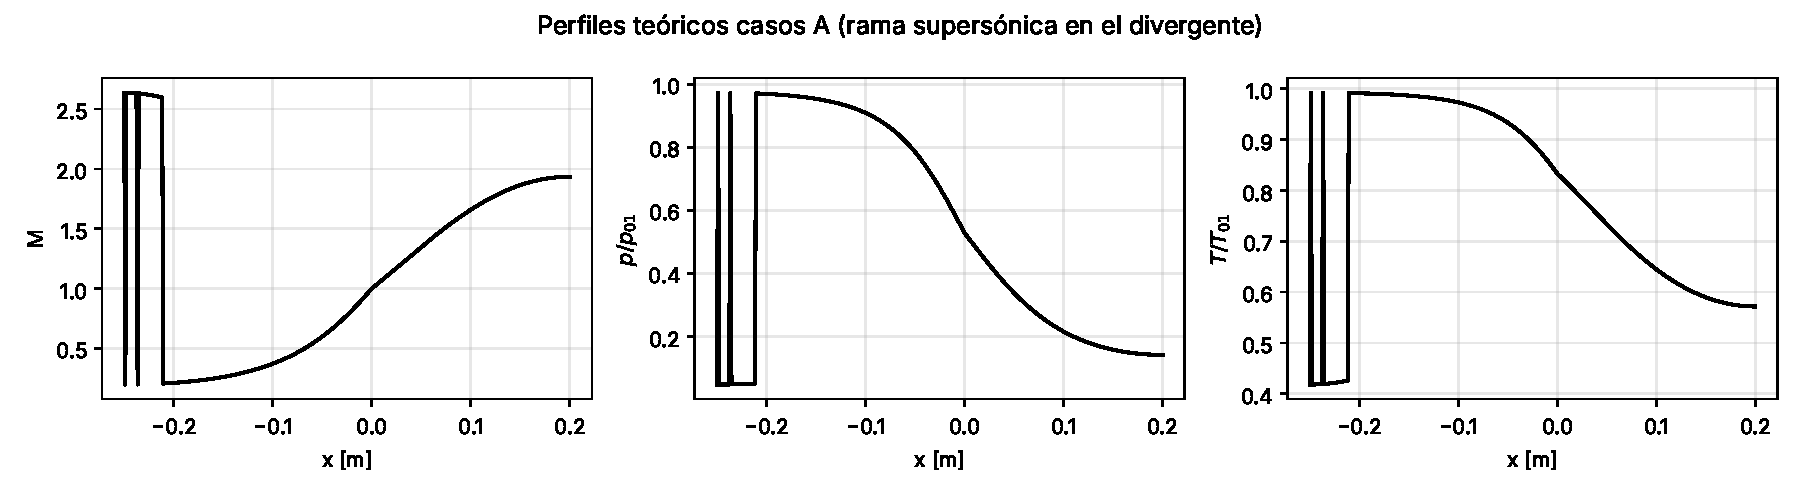
\includegraphics[width=\textwidth]{memoria/figuras/teoria_perfiles_A.pdf}
\caption{Perfiles teóricos del caso A con la $A(x)$ real.}\label{m:fig:perfA}\end{figure}

\subsubsection{Caso S: subsónico no estrangulado}
Con $p_B=\pBS$~kPa ($p_B/p_{01}=\pBSr$, mayor que el límite $\pbSubLim$) la garganta no es sónica, por lo que $A^*\ne A_t$
y hay que \textbf{determinar $A^*$ a partir de la salida}. El flujo es isentrópico y subsónico en toda la tobera y
$p_e=p_B$ (salida subsónica, presión de salida = contrapresión).

\textbf{Paso 1.} Mach de salida con \eqref{m:eq:Mdep}: $M_e=\sqrt{\tfrac{1}{k}\left[(p_{01}/p_B)^{(\gamma-1)/\gamma}-1\right]}=\MeS$.

\textbf{Paso 2.} Cociente de áreas en la salida con \eqref{m:eq:AM}: $A_e/\As=\AeAsS$.

\textbf{Paso 3.} Área crítica relativa a la garganta: $A_t/\As=(A_e/\As)/(A_e/A_t)=\AeAsS/\ARr=\AtAsS$ ($>1$:
la garganta es \emph{más grande} que el área crítica, es decir, subsónica). Equivalentemente $\As/A_t=\AsAtS$.

\textbf{Paso 4.} Mach en la garganta: se resuelve \eqref{m:eq:AM} (rama subsónica) con $a=A_t/\As=\AtAsS$ por Newton (tabla~\ref{m:tab:nS}): $M_t=\MtS<1$.

\textbf{Paso 5.} Gasto: $\dot m=\dot m_{\rm max}\cdot\As/A_t=\mdotsemi\times\AsAtS=\mdotS$~kg/s (semidominio): menor que el bloqueado.

\textbf{Paso 6.} $T_e=T_{01}\,(1+kM_e^2)^{-1}=\TeS$~K y $V_e=M_e\sqrt{\gamma RT_e}=\VeS$~m/s. Los perfiles $M(x)$ salen de resolver \eqref{m:eq:AM}
con $A(x)/\As=(A(x)/A_t)(A_t/\As)=(h/h_t)\,\AtAsS$ en la rama subsónica.

\begin{table}[H]\centering\small
\caption{Newton para $M_t$ del caso S ($A/\As=\AtAsS$, $M_0=0.5$).}\label{m:tab:nS}
\begin{tabular}{rccc}
\toprule
$n$ & $M_n$ & $f(M_n)$ & $\Delta M_n$ \\
\midrule
0 & 0.5000000000 & 2.209e-01 & 1.154e-01 \\
1 & 0.6154235235 & 5.170e-02 & 4.707e-02 \\
2 & 0.6624899194 & 5.426e-03 & 6.198e-03 \\
3 & 0.6686882498 & 8.160e-05 & 9.609e-05 \\
4 & 0.6687843363 & 1.928e-08 & 2.272e-08 \\
5 & 0.6687843590 & 1.110e-15 & 1.308e-15 \\
\bottomrule
\end{tabular}\end{table}

\subsubsection{Caso C: choque normal interno}
\textbf{Datos:} $p_B=\pBC$~kPa ($p_B/p_{01}=\pBCr$, dentro del intervalo $[\pbShockExit,\pbSubLim]$ de choque interno). La garganta es sónica
($A^*_1=A_t$); el choque se ubica donde las condiciones aguas abajo producen exactamente la presión de salida $p_B$.

\textbf{Formulación.} Sea $\Msone$ el Mach justo antes del choque. Aguas abajo el flujo es isentrópico y subsónico hasta la salida, con $p_e=p_B$ (salida subsónica).
La secuencia que liga $\Msone$ con $p_B/p_{01}$ es:
\begin{enumerate}[label=(\roman*)]
\item $\sigma(\Msone)=p_{02}/p_{01}$ con \eqref{m:eq:sigma};
\item área crítica posterior: $A^*_2=A_t/\sigma$ \eqref{m:eq:Astar2}, de modo que $A_e/A^*_2=(A_e/A_t)\,\sigma=\ARr\,\sigma$;
\item $M_e$ subsónico: raíz subsónica de $A/\As(M_e)=\ARr\,\sigma$ \eqref{m:eq:AM};
\item $p_e/p_{01}=\sigma\cdot p/p_0(M_e)$ \eqref{m:eq:prho}, que debe igualar $p_B/p_{01}$.
\end{enumerate}
Así, la incógnita es la raíz de la ecuación escalar
\begin{equation}
F(\Msone)\equiv\sigma(\Msone)\;\frac{p}{p_0}\!\Big|_{M_e(\sigma)}-\frac{p_B}{p_{01}}=0,\qquad 1<\Msone<M_e^{\rm sup}=\MeSup. \label{m:eq:F}
\end{equation}
No tiene solución cerrada (contiene dos inversiones implícitas), por lo que se resuelve numéricamente.

\textbf{Evaluación manual de $F$ en un valor de prueba, $\Msone=\MtrialA$:}
\begin{itemize}[leftmargin=2em]
\item $r=\dfrac{2.4\cdot(\MtrialA)^2}{0.4\cdot(\MtrialA)^2+2}=\rTr$;\quad $\Pi=1+\dfrac{2.8}{2.4}((\MtrialA)^2-1)=\PiTr$;\quad $M_{s2}=\MIITr$.
\item $\sigma=r^{3.5}\,\Pi^{-2.5}=(\rpow)(\Pipow)=\sgTr$.
\item $A_e/A^*_2=\ARr\cdot\sgTr=\AeAdosTr$; raíz subsónica (Newton): $M_e=\MeTr$.
\item $p/p_0=(1+0.2\cdot(\MeTr)^2)^{-3.5}=\prTr$ y $p_e/p_{01}=\sgTr\times\prTr=\pBeTr$.
\item $F=\pBeTr-\pBCr=\FTr>0$.
\end{itemize}
En los extremos del intervalo: $F(1^+)=\FaExt$ y $F(M_e^{\rm sup})=\FbExt$; $F$ cambia de signo y es decreciente
(figura~\ref{m:fig:F}), por lo que existe una única raíz.

\textbf{Método: bisección.} Se elige bisección (confiable y simple de justificar, sin derivadas): partiendo de $[a_0,b_0]=[1^+,M_e^{\rm sup}]$ se toma el punto medio
$m_n=(a_n+b_n)/2$; si $F(m_n)>0$ la raíz está a la derecha ($a_{n+1}=m_n$), si no a la izquierda ($b_{n+1}=m_n$). Cada iteración reduce el intervalo a la mitad y la
iteración termina cuando $b_n-a_n<10^{-12}$ (\nbis\ iteraciones, tabla~\ref{m:tab:bis}). Dentro de cada evaluación de $F$ se resuelve el paso (iii) con Newton.

\begin{figure}[H]\centering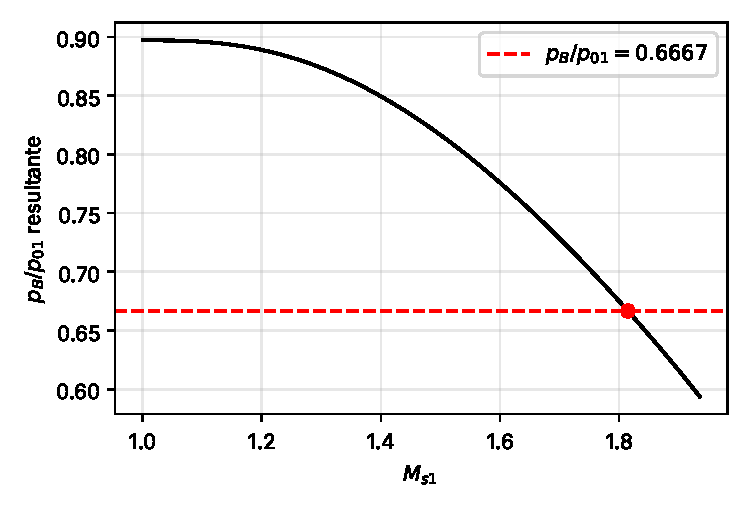
\includegraphics[width=.55\textwidth]{memoria/figuras/F_choque.pdf}
\caption{Presión de salida resultante $p_B/p_{01}$ en función de $M_{s1}$; la intersección con $p_B/p_{01}=\pBCr$ da la solución.}\label{m:fig:F}\end{figure}

\begin{center}\small
\captionof{table}{Bisección de $F(M_{s1})=0$ para el caso C.}\label{m:tab:bis}
\begin{tabular}{rcccc}
\toprule
$n$ & $a_n$ & $b_n$ & $M_{s1}^{(n)}=(a_n+b_n)/2$ & $F(M_{s1}^{(n)})$ \\
\midrule
0 & 1.00000100 & 1.93525761 & 1.46762930 & +1.614e-01 \\
1 & 1.46762930 & 1.93525761 & 1.70144346 & +6.103e-02 \\
2 & 1.70144346 & 1.93525761 & 1.81835053 & -2.033e-03 \\
3 & 1.70144346 & 1.81835053 & 1.75989699 & +3.045e-02 \\
4 & 1.75989699 & 1.81835053 & 1.78912376 & +1.445e-02 \\
5 & 1.78912376 & 1.81835053 & 1.80373715 & +6.265e-03 \\
6 & 1.80373715 & 1.81835053 & 1.81104384 & +2.131e-03 \\
7 & 1.81104384 & 1.81835053 & 1.81469719 & +5.254e-05 \\
8 & 1.81469719 & 1.81835053 & 1.81652386 & -9.892e-04 \\
9 & 1.81469719 & 1.81652386 & 1.81561052 & -4.681e-04 \\
10 & 1.81469719 & 1.81561052 & 1.81515385 & -2.077e-04 \\
11 & 1.81469719 & 1.81515385 & 1.81492552 & -7.758e-05 \\
12 & 1.81469719 & 1.81492552 & 1.81481135 & -1.251e-05 \\
13 & 1.81469719 & 1.81481135 & 1.81475427 & +2.002e-05 \\
14 & 1.81475427 & 1.81481135 & 1.81478281 & +3.752e-06 \\
15 & 1.81478281 & 1.81481135 & 1.81479708 & -4.380e-06 \\
16 & 1.81478281 & 1.81479708 & 1.81478995 & -3.138e-07 \\
17 & 1.81478281 & 1.81478995 & 1.81478638 & +1.719e-06 \\
18 & 1.81478638 & 1.81478995 & 1.81478816 & +7.027e-07 \\
19 & 1.81478816 & 1.81478995 & 1.81478905 & +1.945e-07 \\
20 & 1.81478905 & 1.81478995 & 1.81478950 & -5.967e-08 \\
21 & 1.81478905 & 1.81478950 & 1.81478928 & +6.740e-08 \\
22 & 1.81478928 & 1.81478950 & 1.81478939 & +3.868e-09 \\
23 & 1.81478939 & 1.81478950 & 1.81478944 & -2.790e-08 \\
24 & 1.81478939 & 1.81478944 & 1.81478942 & -1.202e-08 \\
25 & 1.81478939 & 1.81478942 & 1.81478940 & -4.074e-09 \\
26 & 1.81478939 & 1.81478940 & 1.81478940 & -1.027e-10 \\
27 & 1.81478939 & 1.81478940 & 1.81478939 & +1.883e-09 \\
28 & 1.81478939 & 1.81478940 & 1.81478939 & +8.901e-10 \\
29 & 1.81478939 & 1.81478940 & 1.81478940 & +3.937e-10 \\
30 & 1.81478940 & 1.81478940 & 1.81478940 & +1.455e-10 \\
31 & 1.81478940 & 1.81478940 & 1.81478940 & +2.143e-11 \\
32 & 1.81478940 & 1.81478940 & 1.81478940 & -4.062e-11 \\
33 & 1.81478940 & 1.81478940 & 1.81478940 & -9.595e-12 \\
34 & 1.81478940 & 1.81478940 & 1.81478940 & +5.915e-12 \\
35 & 1.81478940 & 1.81478940 & 1.81478940 & -1.840e-12 \\
36 & 1.81478940 & 1.81478940 & 1.81478940 & +2.037e-12 \\
37 & 1.81478940 & 1.81478940 & 1.81478940 & +9.892e-14 \\
38 & 1.81478940 & 1.81478940 & 1.81478940 & -8.706e-13 \\
39 & 1.81478940 & 1.81478940 & 1.81478940 & -3.858e-13 \\
\bottomrule
\end{tabular}\end{center}

\textbf{Resultado.} $\Msone=\MsI$. Con ese valor:
\begin{itemize}[leftmargin=2em]
\item Relaciones del choque: $r=\rrC$; $p_2/p_1=1+\tfrac{2.8}{2.4}(\MsCsq-1)=\pIIpI$; $M_{s2}^2=\numMdos/\denMdos\Rightarrow M_{s2}=\MsII$.
\item $\sigma=p_{02}/p_{01}=\pdospu$ (equivale a $p_{02}=\pdos$~kPa); $A^*_2=A_t/\sigma=\AstarC\,A_t$.
\item Área del choque: $A_s/A_t=A/\As(M_{s1})=\AsAt$.
\item \textbf{Posición del choque} con \eqref{m:eq:xinv}: $\cos(\pi x_s/L_d)=1-2(\AsAt-1)/(\ARr-1)$, y entonces
$x_s=\xsC$~m, es decir $\boxed{x_s/L_d=\xsLd}$ (semialtura de pared $h(x_s)=\hxs$~m).
\item Estados antes/después: $p_{s1}=\pIkPa$~kPa ($p_{s1}/p_{01}=\pIrel$), $T_{s1}=\TIK$~K; $p_{s2}=\pIIkPa$~kPa, $T_{s2}=\TIIK$~K.
\item Salida: $A_e/A^*_2=\AeAstarC$, $M_e=\MeC$, $p_e=\pBC$~kPa (por construcción), $T_e=\TeC$~K, $V_e=\VeC$~m/s.
\end{itemize}

\begin{figure}[H]\centering
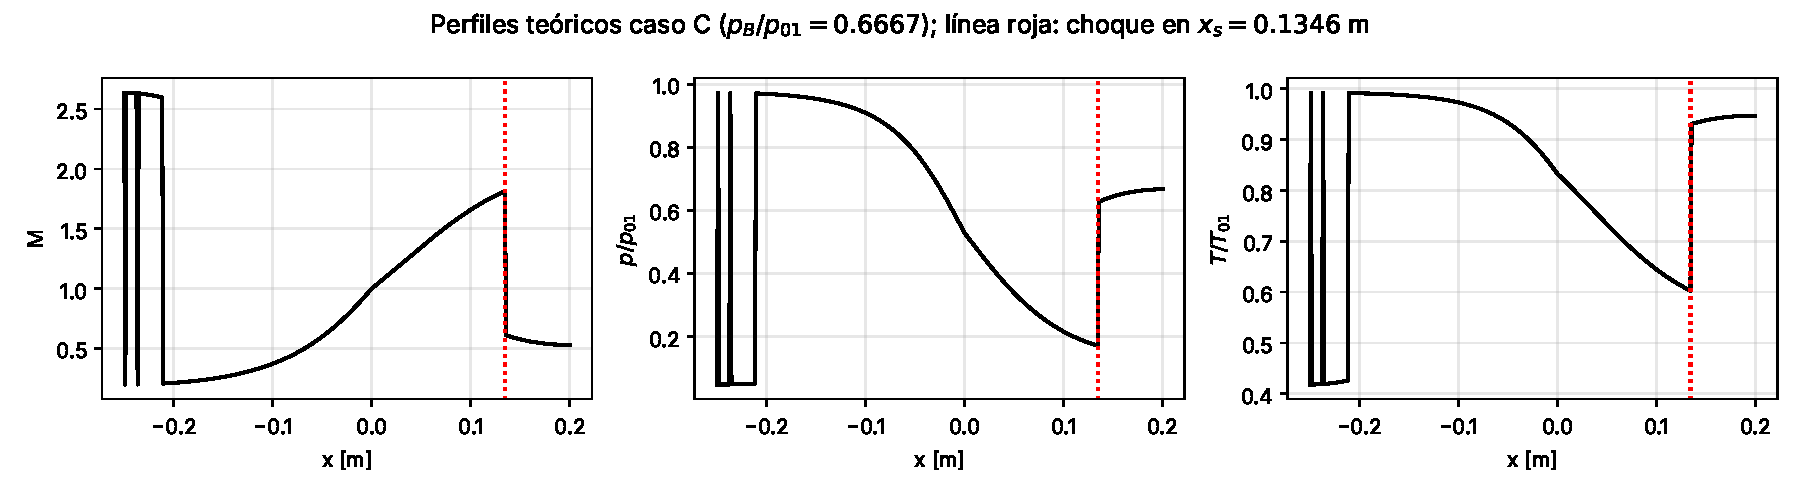
\includegraphics[width=\textwidth]{memoria/figuras/teoria_perfiles_C.pdf}
\caption{Perfiles teóricos del caso C con la $A(x)$ real. El salto en $x_s$ es el choque normal.}\label{m:fig:perfC}\end{figure}

\subsubsection{Cálculo manual completo en una estación del divergente ($x=\xAs$~m, caso A)}
\begin{enumerate}[leftmargin=2em]
\item Altura de pared con \eqref{m:eq:hdiv}: $\cos(\pi x/L_d)=\cos(\pi\cdot\xAs/\Ldd)=\cosA$, por lo que
$h=h_t+\tfrac{h_e-h_t}{2}(1-\cosA)=\hth+\tfrac{\heh-\hth}{2}=\hAs$~m.
\item Cociente de áreas: $A/A_t=\hAs/\hth=\aAs$; garganta sónica $\Rightarrow\As=A_t$, por lo que $A/\As=\aAs$.
\item Se resuelve \eqref{m:eq:AM} (rama supersónica) con Newton, $M_0=1.5$ (tabla~\ref{m:tab:nest}): $M=\MAs$.
\item $p/p_{01}=(1+0.2\cdot(\MAs)^2)^{-3.5}=\pAs$, es decir $p=\pAsPa$~kPa.
\item $T/T_{01}=(1+0.2\cdot(\MAs)^2)^{-1}=\TAs$, es decir $T=\TAsK$~K.
\end{enumerate}
\begin{table}[H]\centering\small
\caption{Newton para la estación $x=\xAs$~m ($A/\As=\aAs$, $M_0=1.5$).}\label{m:tab:nest}
\begin{tabular}{rccc}
\toprule
$n$ & $M_n$ & $f(M_n)$ & $\Delta M_n$ \\
\midrule
0 & 1.5000000000 & -1.238e-01 & 1.832e-01 \\
1 & 1.6831961950 & 2.197e-02 & -2.390e-02 \\
2 & 1.6592927206 & 3.941e-04 & -4.448e-04 \\
3 & 1.6588479422 & 1.353e-07 & -1.528e-07 \\
4 & 1.6588477894 & 1.577e-14 & -1.780e-14 \\
\bottomrule
\end{tabular}\end{table}
Para una estación del convergente, p.~ej.\ $x=\xBs$~m: $h=\hBs$~m, $A/A_t=\aBs$ y la raíz subsónica da $M=\MBs$, $p/p_{01}=\pBs$, $T/T_{01}=\TBs$.

%=====================================================================
\subsection{Definición de métricas de error}
%=====================================================================
Para comparar CFD con teoría se usan las definiciones siguientes (se aplican a magnitudes no nulas):
\begin{align}
\varepsilon_\phi&=\frac{|\phi_{\rm CFD}-\phi_{\rm teo}|}{|\phi_{\rm teo}|}\times100\,\%&&\text{(error relativo puntual o de estación)}\\
\bar\varepsilon_\phi&=\frac1N\sum_{i=1}^{N}\frac{|\phi_{{\rm CFD},i}-\phi_{{\rm teo},i}|}{|\phi_{{\rm teo},i}|}\times100\,\%&&\text{(error medio a lo largo del eje)}\\
\varepsilon_{x_s}&=\frac{|x_{s,\rm CFD}-x_{s,\rm teo}|}{L_d}\times100\,\%&&\text{(error de posición del choque, normalizado con $L_d$)}\\
\delta_{\dot m}&=\frac{\dot m_{\rm sal}-\dot m_{\rm ent}}{\dot m_{\rm ent}}\times100\,\%&&\text{(desbalance de masa)}
\end{align}
La posición del choque en el CFD se define como la coordenada donde el Mach promediado en el tiempo cruza $M=1$ aguas abajo del pico supersónico
(método fijo para todas las mallas); los estados $M_{s1}$, $M_{s2}$, $p_2/p_1$ y $p_{02}/p_{01}$ se miden en estaciones fuera del espesor numérico del choque
(a una distancia de varias celdas a cada lado). Los valores del CFD se promedian en una ventana temporal posterior al arranque, cuyo efecto se evalúa en la sección de sensibilidad temporal.

%=====================================================================

\subsection{Código de la memoria}\label{m:cod}
%=====================================================================
El siguiente módulo implementa exactamente las ecuaciones de las secciones anteriores y es la fuente de todos los números y tablas de este documento.
\lstinputlisting[caption={\texttt{teoria\_tobera.py}}]{memoria/codigo/teoria_tobera.py}

\subsection*{Referencias de la memoria}
\begin{enumerate}[leftmargin=2em]
\item J.~D. Anderson Jr., \emph{Modern Compressible Flow: With Historical Perspective}, 3.ª ed., McGraw-Hill, 2003 (caps.~3--5: ecuaciones isentrópicas, choque normal, flujo en toberas).
\item H.~W. Liepmann y A.~Roshko, \emph{Elements of Gasdynamics}, Dover, 2001.
\item Hoja de actividad y rúbrica, \emph{Proyecto final: simulación de una tobera}, Aerodinámica II (AE604), UACH.
\end{enumerate}
